\documentclass[conference]{IEEEtran}
\IEEEoverridecommandlockouts
\usepackage{cite}
\usepackage{amsmath,amssymb}
\usepackage{graphicx}
\usepackage{textcomp}
\usepackage{booktabs}
\usepackage{url}
\usepackage[caption=false,font=footnotesize]{subfig}
\usepackage{tikz}
\usetikzlibrary{positioning,fit,backgrounds,arrows.meta,calc}

\newcommand{\uV}{\,\textmu V}
\newcommand{\uVrms}{\,\textmu V\textsubscript{rms}}
\newcommand{\uVpp}{\,\textmu V\textsubscript{pp}}
\newcommand{\uA}{\,\textmu A}
\newcommand{\uW}{\,\textmu W}
\newcommand{\um}{\,\textmu m}
\newcommand{\nVrtHz}{\,nV/$\sqrt{\mathrm{Hz}}$}

\begin{document}
\bstctlcite{IEEEexample:BSTcontrol}

\title{Toward Electrode-to-Alarm Hardware for Neonatal Seizure Detection: A SKY130 EEG Front End and Hardware-Exact Gradient-Boosted Trees on an FPGA SoC}

\author{\IEEEauthorblockN{A Sai Chaithr Choudary}
\IEEEauthorblockA{Department of Electronics and Communication Engineering\\
National Institute of Technology Warangal, India\\
chaithr45@gmail.com}}

\maketitle

\begin{abstract}
Most neonatal seizures have no visible clinical signs and are recognised only by continuous EEG review. We present both hardware halves of a neonatal seizure monitor and analyse the interface that would join them. The analog front end (AFE) is a capacitive-feedback EEG amplifier in the open SKY130 process on a 161$\times$226\um{} (1$\times$2) Tiny Tapeout tile. In post-layout simulation it has 37.8\,dB of gain, a pass band from below 0.15\,Hz to 22\,kHz, 2.95\uVrms{} of input noise from 0.5 to 100\,Hz and over 81\,dB of PSRR at 50\,Hz, at 15.7\uA{} from 1.8\,V. Post-layout simulation of its code-generated layout found two parasitic couplings that DRC, LVS and the shuttle precheck had passed. The detector is implemented in the programmable logic of an AMD Kria KV260 and scores 108 integer features with 100 gradient-boosted trees trained on the hardware's own integer features, so the evaluated and the implemented detectors are identical. Under pre-registered nested patient-wise cross-validation on the 79 neonates of the public Helsinki dataset it finds 47.8\% of seizures at 0.91 false alarms per hour; it is bit-exact with its Python golden model through the AXI interface and uses 9,592 LUTs and 62 DSP slices at 100\,MHz. Digital re-referencing of single-ended AFE channels leaves 3.5\uVrms{} of AFE noise in the detector's 0.5--20\,Hz band and a mismatch-limited midband CMRR of about 62\,dB. Both halves are pre-silicon, and the two have not yet been connected.
\end{abstract}

\begin{IEEEkeywords}
Neonatal seizure detection, EEG analog front end, SKY130, Tiny Tapeout, FPGA, gradient-boosted trees, post-layout simulation, bit-exact verification
\end{IEEEkeywords}

\section{Introduction}

Seizures in newborns are frequently subclinical. In a video-EEG study, only 34\% of 526 electrographic neonatal seizures showed clinical signs, and only 9\% were recognised and documented by staff~\cite{murray2008}. Reliable recognition therefore needs continuous multichannel EEG read by an expert, which most neonatal units cannot provide day and night. Machine-learning decision support has reached a randomised trial~\cite{pavel2020}.

\begin{figure*}[t]
\centering
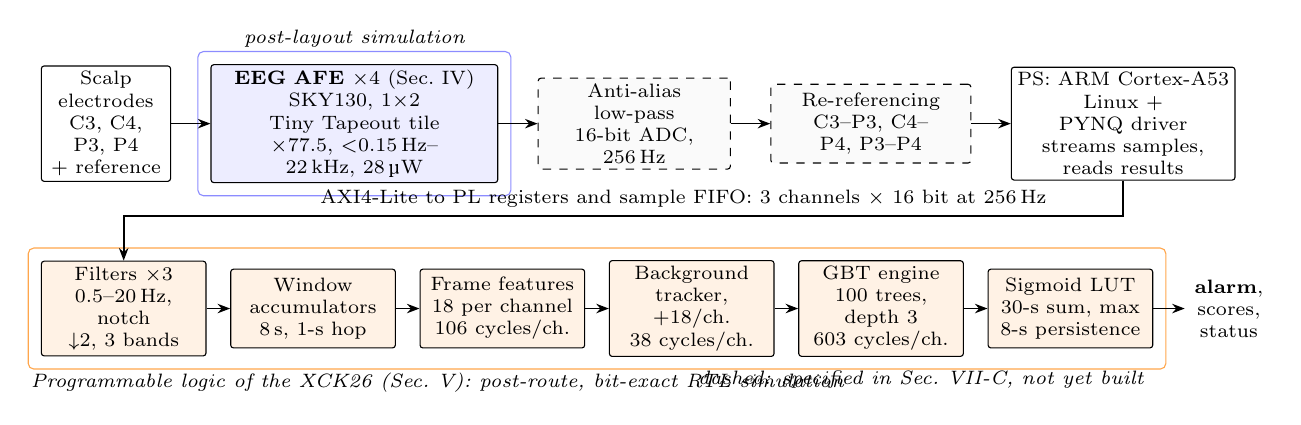
\begin{tikzpicture}[font=\scriptsize, node distance=4mm,
  box/.style={draw, rounded corners=1pt, align=center, inner sep=2pt, minimum height=10mm, fill=white},
  ana/.style={box, fill=blue!7},
  dig/.style={box, fill=orange!10, text width=19.5mm},
  fut/.style={box, dashed, fill=gray!4},
  ar/.style={-{Stealth[length=1.6mm]}, semithick}]
\node[box, text width=15mm] (el) {Scalp electrodes\\C3, C4, P3, P4\\+ reference};
\node[ana, right=5mm of el, text width=35mm] (afe) {\textbf{EEG AFE} $\times$4 (Sec.~IV)\\SKY130, 1$\times$2 Tiny Tapeout tile\\$\times$77.5, $<$0.15\,Hz--22\,kHz, 28\uW};
\node[fut, right=5mm of afe, text width=23mm] (adc) {Anti-alias low-pass\\16-bit ADC, 256\,Hz};
\node[fut, right=5mm of adc, text width=24mm] (rr) {Re-referencing\\C3--P3, C4--P4, P3--P4};
\node[box, right=5mm of rr, text width=27mm] (ps) {PS: ARM Cortex-A53\\Linux + PYNQ driver\\streams samples, reads results};
\node[dig, below=10mm of el.south west, anchor=north west] (f1) {Filters $\times$3\\0.5--20\,Hz, notch\\$\downarrow$2, 3 bands};
\node[dig, right=3mm of f1] (f2) {Window\\accumulators\\8\,s, 1-s hop};
\node[dig, right=3mm of f2] (f3) {Frame features\\18 per channel\\106 cycles/ch.};
\node[dig, right=3mm of f3] (f4) {Background\\tracker, +18/ch.\\38 cycles/ch.};
\node[dig, right=3mm of f4] (f5) {GBT engine\\100 trees, depth 3\\603 cycles/ch.};
\node[dig, right=3mm of f5] (f6) {Sigmoid LUT\\30-s sum, max\\8-s persistence};
\node[right=4mm of f6, align=center] (al) {\textbf{alarm},\\scores,\\status};
\draw[ar] (el) -- (afe);
\draw[ar] (afe) -- (adc);
\draw[ar] (adc) -- (rr);
\draw[ar] (rr) -- (ps);
\draw[ar] (ps.south) -- ++(0,-4.5mm) -| node[pos=0.22, above=-0.5pt] {AXI4-Lite to PL registers and sample FIFO: 3 channels $\times$ 16 bit at 256\,Hz} (f1.north);
\foreach \a/\b in {f1/f2, f2/f3, f3/f4, f4/f5, f5/f6, f6/al} \draw[ar] (\a) -- (\b);
\begin{scope}[on background layer]
\node[draw=blue!45, rounded corners=2pt, fit=(afe), inner sep=1.6mm,
      label={[font=\scriptsize\itshape, anchor=south, inner sep=1pt]north:post-layout simulation}] {};
\node[draw=orange!70, rounded corners=2pt, fit=(f1)(f6), inner sep=1.6mm,
      label={[font=\scriptsize\itshape, anchor=north west, inner sep=1pt]south west:Programmable logic of the XCK26 (Sec.~V): post-route, bit-exact RTL simulation}] {};
\end{scope}
\node[font=\scriptsize\itshape, anchor=north east] at ($(f6.south east)+(0,-1.6mm)$) {dashed: specified in Sec.~VII-C, not yet built};
\end{tikzpicture}
\caption{The monitor: one single-ended AFE per electrode, digital re-referencing, and the detector in the programmable logic (PL), fed by the processing system (PS). Cycle counts are per channel and frame.}
\label{fig:system}
\end{figure*}

A monitor needs an analog front end that amplifies microvolt EEG and a detector that turns the samples into an alarm, but the two are usually developed apart. Neonatal seizure detectors run as software on workstations~\cite{temko2011,ansari2019,oshea2020}; seizure-detection hardware has largely targeted adult and paediatric data~\cite{verma2010,busia2025,vittimberga2025}, often with patient-specific training~\cite{verma2010}, which a newborn cannot provide; and biopotential amplifiers are reported by circuit figures of merit~\cite{harrison2003,steyaert1987}, without the band, montage and converter of a particular detector. Both halves also have a gap between the design that is evaluated and the one that is built. A model trained in floating point and quantised afterwards silently changes its decisions, evaluations that tune and test on the same patients overstate performance~\cite{varma2006}, and an amplifier layout that passes design-rule (DRC) and layout-versus-schematic (LVS) checks can still differ from its schematic through parasitic coupling.

This paper presents both halves and the interface between them. Its contributions are:
\begin{itemize}
\item an EEG AFE in SKY130~\cite{sky130} on a 1$\times$2 Tiny Tapeout~\cite{tinytapeout} tile, whose code-generated layout is verified up to post-layout simulation, which found two defects that DRC and LVS cannot see;
\item a three-channel neonatal seizure detector in FPGA logic, trained on the hardware's exact integer features and bit-exact from the Python reference to the AXI-attached RTL;
\item a pre-registered, nested patient-wise evaluation comparing nine detectors against their hardware cost;
\item an interface analysis that states what the present AFE can and cannot support.
\end{itemize}
To our knowledge, this is the first neonatal seizure detector implemented in FPGA logic and evaluated patient-independently on a public neonatal dataset. The AFE design files, scripts and results are public.\footnote{\url{https://github.com/chaithr45/tt-eeg-afe}}

\section{Related Work}

Software neonatal detectors reached about 89\% of seizures at one false detection per hour with support vector machines~\cite{temko2011}, 77\% at 0.9 false alarms per hour with a CNN~\cite{ansari2019} and an AUC of 98.5\% with a fully convolutional network~\cite{oshea2020}. The public Helsinki dataset~\cite{stevenson2019} enabled a classifier on a Raspberry Pi~\cite{nagarajan2021}, without a stated patient-independent protocol or false-alarm rate. In hardware, a micropower EEG acquisition SoC extracted features for a patient-specific detector~\cite{verma2010}, an FPGA spiking neural network reached 99.3\% accuracy on the paediatric CHB-MIT database~\cite{busia2025}, and a threshold algorithm was designed for low-complexity hardware~\cite{vittimberga2025}; none targets neonates. The capacitive-feedback amplifier with MOS pseudo-resistors~\cite{harrison2003} remains the standard AC-coupled low-noise topology and the noise efficiency factor (NEF)~\cite{steyaert1987} its usual figure of merit; clinical EEG converters reach 1\uVpp{} in a 70-Hz band~\cite{ads1299}.


\section{System Overview}

Fig.~\ref{fig:system} shows the intended monitor. Four scalp electrodes (C3, C4, P3, P4) are each amplified single-ended against a common reference electrode by one AFE. Each AFE occupies one 1$\times$2 tile with two analog pins, and each Tiny Tapeout chip carries one copy of a design, so four chips give four channels. The AFE outputs are digitised at 256\,Hz, the sampling rate of the Helsinki recordings, and the detector's bipolar derivations C3--P3, C4--P4 and P3--P4 are formed by subtraction. The processing system (PS) of the KV260 streams them as 16-bit samples to the detector in the programmable logic (PL) and reads alarms and scores back. The AFE (Section~IV) and the detector (Section~V) are complete designs; the converter and the re-referencing step are specified in Section~VII-C but not built, and the halves have not yet been run together.

\section{Analog Front End}

\subsection{Circuit}

Fig.~\ref{fig:sch}(a) shows the amplifier. The input ua[0] is AC-coupled through $C_1 = 11.9$\,pF to the inverting input of the operational transconductance amplifier (OTA) A1, with $C_2 = 154$\,fF, a pseudo-resistor PR1 and a reset switch S1 in feedback, so the midband gain is set by $C_1/C_2$: 77.5\,V/V (37.8\,dB) in simulation~\cite{harrison2003}. The non-inverting input sees $C_1'$ to ground and $C_2' \parallel$ PR2 $\parallel$ S2 to the reference VREF; because $C_1'$ goes to ground rather than to the signal, VREF noise reaches the output with a gain of about 1 instead of 78, so a simple on-chip reference suffices. Each pseudo-resistor is two back-to-back pairs of 0.42/1\um{} PMOS devices in series, about $2\times10^{13}\,\Omega$ at 37\,\textdegree C, which places $f_L = 1/(2\pi R_{PR} C_2)$ at 0.04--0.14\,Hz over process corners at 37\,\textdegree C, well below the detector's 0.5-Hz band edge. Pseudo-resistors alone take about 15\,s to settle at power-up and stay saturated for seconds after a large artifact, so the reset input rst (ui\_in[0]) closes S1 and S2 and ties the pseudo-resistors' internal nodes; a 10-ms pulse returns the output to VREF within 1\,mV after a 20-mV artifact.

A1 (Fig.~\ref{fig:sch}(b)) is a two-stage Miller OTA. The PMOS input pair (150/8\um{} per side, 2\uA{} each) drives an NMOS mirror whose devices are each three 7/20\um{} transistors in series. In a first design the mirror's $1/f$ noise dominated, giving 22\uVrms; because its input-referred contribution falls roughly as $1/L^2$, the 60-\textmu m effective length brought the total to 3.5\uVrms; enlarging $C_1$ from 8 to 11.9\,pF, which lowers the noise gain $(C_1 + C_2 + C_\mathrm{in})/C_1$ set by the 3-pF input-pair capacitance, together with a wider input pair brought it to 2.9\uVrms. The second stage is an NMOS common-source stage at 10\uA{} with $C_c = 2$\,pF and $R_z = 20$\,k$\Omega$. The open-loop gain is 99\,dB; with a feedback factor of about 1/80 the loop phase margin is 86\textdegree, so A1 drives the pin and a 15-pF load without a buffer.

A subthreshold beta-multiplier with start-up supplies 0.5\uA{} per PMOS unit cell, and VREF is a weak-inversion NMOS diode at one unit current, 0.45\,V (0.39--0.50\,V over corners), which keeps the tail transistor saturated with a margin of at least 0.04\,V (slow corner, 0\,\textdegree C, 1.71\,V). The circuit draws 15.7\uA{} from 1.8\,V (28\uW), bias and reference included.

\begin{figure}[t]
\centering
\subfloat[]{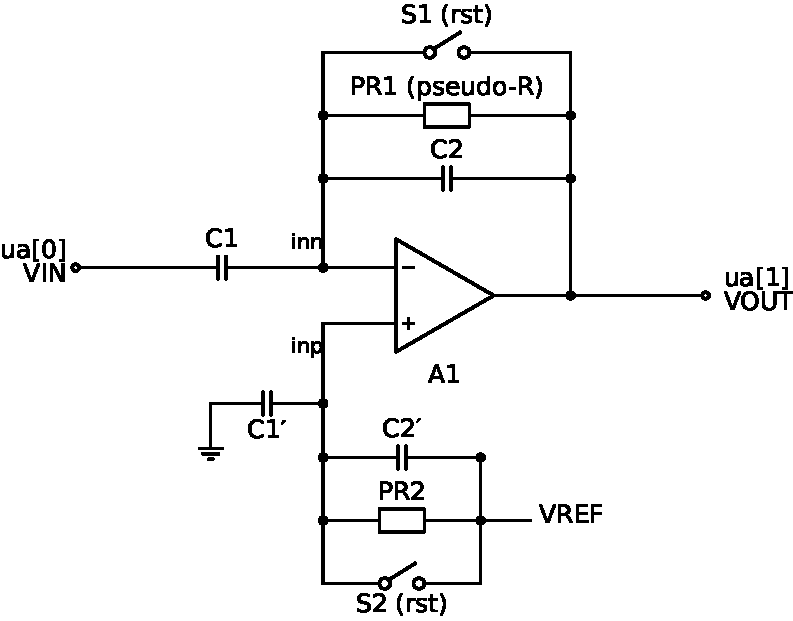
\includegraphics[width=0.74\columnwidth]{figs/afe_top.pdf}}\\[-1mm]
\subfloat[]{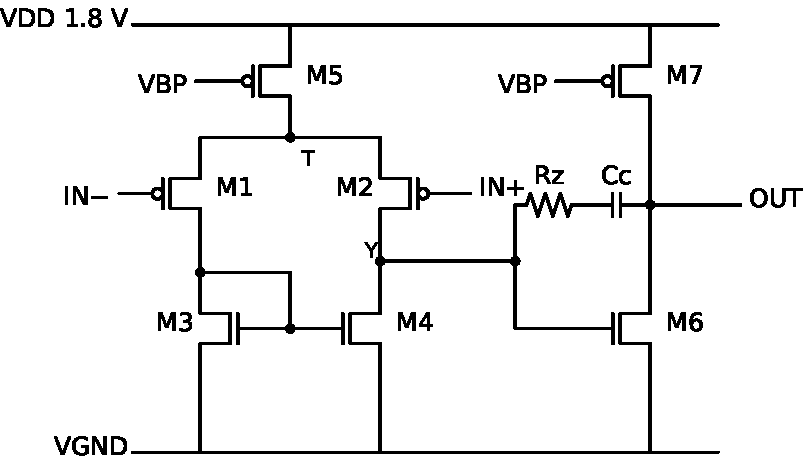
\includegraphics[width=0.76\columnwidth]{figs/afe_ota.pdf}}
\caption{AFE schematic. (a) Capacitive-feedback amplifier: $C_1 = C_1' = 11.9$\,pF, $C_2 = C_2' = 154$\,fF; PR, MOS pseudo-resistor; S1, S2, reset switches driven by rst = ui\_in[0]. (b) Two-stage Miller OTA A1; VBP comes from the beta-multiplier; M3 and M4 are each three 7/20\um{} devices in series.}
\label{fig:sch}
\end{figure}

\subsection{Layout as Code}

The layout (Fig.~\ref{fig:layout}) is generated by Python scripts that emit Magic~\cite{edatools} commands, one per block (devices, pseudo-resistor, OTA, bias, core and tile). One build script rebuilds the tile from scratch, runs Magic DRC and Netgen LVS on the core and on the whole tile, and extracts parasitics; a rebuild reproduces the GDS exactly. The 28\,pF of MIM capacitance takes about 40\% of the tile, and the tile passes the Tiny Tapeout precheck (Magic and KLayout rules, pins, forbidden layers) locally and in continuous integration.

\begin{figure}[t]
\centering
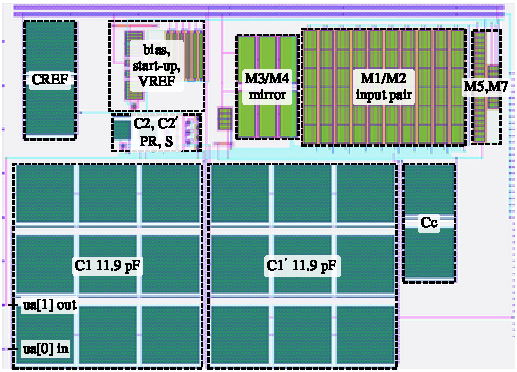
\includegraphics[width=0.9\columnwidth]{figs/layout_annotated.pdf}
\caption{Layout of the 161$\times$225.8\um{} (1$\times$2) Tiny Tapeout tile, rotated 90\textdegree: the shuttle's power stripes run along the top and the analog pins on the left. Dashed boxes mark the blocks; $C_c$ and CREF are 2-pF MIM capacitors.}
\label{fig:layout}
\end{figure}

\subsection{Post-Layout Simulation}

The extracted core, with all parasitic capacitances, is simulated against the schematic in one test bench: the on-chip bias, a 500\,$\Omega$\,+\,5\,pF model of each shuttle analog pin path and a 15\,pF\,$\parallel$\,1\,M$\Omega$ load, with both the classic and the newer continuous SKY130 model sets. In AC and noise runs the pseudo-resistors are linear $1.3\times10^{13}$-$\Omega$ resistors with thermal noise; in transient runs they are transistors.

The first complete layout passed DRC, LVS and the precheck, but post-layout simulation showed two defects. First, the gain was 0.56\,dB high (82.7\,V/V): the output and the non-inverting input were coupled by 12\,fF, 8\,fF of it from a 150-\textmu m trunk run 1\um{} apart and 4\,fF inside the OTA, which fed about 7\% of the $C_2$ feedback back as positive feedback. A ground shield track between the two trunks removed the error and restored the 22.4-kHz bandwidth, which had dropped to 19.9\,kHz. Second, the 50-Hz PSRR was 77\,dB instead of 96\,dB: the topmost input-pair row, an inverting-input row, sat 1.5\um{} from the M7 row, coupling 0.45\,fF from the supply and 0.9\,fF from the PMOS bias line, which follows the supply, onto the inverting input only. Another 1.5\um{} of spacing and a metal-1 line on the tail node between the rows cut both to 0.14\,fF and raised the PSRR to 85.6\,dB; the remaining 11\,dB to the schematic, from drain wiring over the input gates, is accepted (PSRR $>$81\,dB in every corner). Neither defect violates a rule or changes connectivity, so only extraction and simulation could find them.

\section{Seizure Detector}

\subsection{Data and Evaluation Protocol}

The Helsinki dataset~\cite{stevenson2019} contains EEG from 79 term neonates (111.9\,h) sampled at 256\,Hz and annotated second by second by three experts. We use the derivations C3--P3, C4--P4 and P3--P4 and take the experts' majority as the reference: 492 seizures in 46 neonates. A first threshold detector built in hardware owed its 14.2\% sensitivity to one neonate, and its line length separated seizure from non-seizure within neonates (AUC 0.74) but barely across them (0.52), which motivated background normalisation, a trained classifier and the following protocol.

All results use nested patient-wise cross-validation: the neonates form five outer folds, each tested once, and every choice of features, model and threshold is made by four-fold cross-validation inside the training neonates. The threshold targets 0.5, 1 or 2 false alarms per hour (FA/h) on inner out-of-fold scores, so test neonates never influence it. Success criteria were committed before any result was computed. The model search covered windows, montages, feature sets, smoothing and four model families; a small CNN on raw EEG served as an accuracy reference only. We report event sensitivity (fraction of the 492 seizures detected), FA/h, median per-neonate and pooled AUC and Cohen's $\kappa$ against the expert majority~\cite{cohen1960}, with 95\% confidence intervals from bootstrap resampling of neonates.

\subsection{Filtering and Features}

Ten second-order sections per channel implement a 0.5-Hz high-pass, a 20-Hz low-pass and a 50-Hz notch, decimate to 128\,Hz and split the signal into delta, theta and alpha--beta bands. All 30 sections use the direct form~I (the direct form~II overflowed at the 0.991 pole of the high-pass), 26-bit Q4.22 coefficients, first-order error feedback against deadband and rounding that preserves the high-pass zero at DC; each reuses one multiplier for its five products.

Every second, 18 base features are computed per channel over the last 8\,s: line length~\cite{esteller2001}, absolute and relative energies of the three bands, a spectral entropy from the band energies (no FFT), mean and maximum absolute amplitude, zero-crossing and extrema counts, Hjorth activity, mobility and complexity~\cite{hjorth1970}, Teager energy~\cite{kaiser1990}, crest factor and the envelope's log$_2$ coefficient of variation. Windows are formed from eight 1-s partial sums in block RAM, so an 8-s window costs eight accumulators rather than 1,024 stored samples. Each base feature is paired with a version normalised to a recursively updated per-channel background: 36 features per channel, 108 in total. The definitions were chosen for exact integer evaluation; for example, the envelope variation is a log$_2$ ratio and the 30-s smoother a running sum, neither needing a divider.

\subsection{Classifier and Hardware-Exact Training}

A gradient-boosted tree ensemble~\cite{friedman2001} (scikit-learn HistGradientBoostingClassifier~\cite{pedregosa2011}; 100 trees, depth 3, balanced class weights) scores each channel's 36 features, with one model shared by the three channels. For channel $c$ and frame $t$ the hardware computes
\begin{equation}
z_c(t) = b + \sum_{m=1}^{100} f_m\bigl(x_c(t)\bigr),\quad
S(t) = \max_{c} \sum_{k=0}^{29} \hat\sigma\bigl(z_c(t-k)\bigr),
\end{equation}
where $f_m$ returns the Q16 leaf reached in tree $m$, $b$ is the baseline logit and $\hat\sigma$ a 2,048-entry sigmoid table. The alarm is raised when $S$ has stayed at or above a programmable threshold $\theta$ for 8\,s. The deployed model is refitted on all 79 neonates, with $\theta$ at the 1-FA/h point of the out-of-fold scores.

Post-training quantisation of a floating-point ensemble cannot be made exact: in our first attempt some feature values lay within $10^{-12}$ of a split threshold, and at Q16 resolution 401 of 500,000 node comparisons took a different branch; extra fractional bits reduced but never removed such flips. We therefore define the features in the integer arithmetic of the RTL and train and evaluate the classifier on these integers. Split thresholds become integers that the hardware compares exactly, leaves are stored in Q16, and no standardisation is needed at run time. The integer trees differ from scikit-learn's decision function by at most $1.8\times10^{-4}$ in the logit, and the hardware-exact features track their floating-point counterparts closely (Pearson $r \ge 0.9995$ for 27 of 35 comparable features).

\subsection{Architecture}

The detector is an AXI4-Lite peripheral beside the Zynq UltraScale+ PS, clocked at 100\,MHz. With $f_s = 256$\,Hz the budget between time steps is $f_\mathrm{clk}/f_s = 390{,}625$ cycles, so the design trades latency for area: arithmetic units are shared and sequenced and state is kept in RAM. Once per second the frame calculator, background tracker and tree engine run for each channel in turn, followed by the sigmoid, smoothing and decision steps: 2,399 cycles (24\,\textmu s) in the worst case, against at most 141 cycles for other time steps. All counts are fixed by design, so the worst-case latency is known exactly. The tree engine walks the 100 trees with three integer comparisons per tree and holds the model in two 1,500-word RAMs written over AXI, so a retrained model needs no new bitstream; it uses 162 LUTs and two block RAMs.

\section{Verification}

Each half is checked against one reference (Table~\ref{tab:verif}). For the AFE it is the schematic: the layout must pass DRC, match the schematic netlist in LVS, pass the shuttle precheck and match the schematic's behaviour in post-layout simulation within the specification, with every remaining difference explained; this step found the defects of Section~IV-C. For the detector any difference counts as a defect. Its reference is a Python golden model that follows the RTL's operation order; every block and the full system are simulated in Vivado xsim against it. The same integer model supplies the training features, so the evaluated and the implemented detectors are the same.

\begin{table}[t]
\caption{Verification of Both Halves}
\label{tab:verif}
\centering
\footnotesize
\setlength{\tabcolsep}{3pt}
\begin{tabular}{@{}lll@{}}
\toprule
Check & Reference & Result \\
\midrule
\multicolumn{3}{@{}l}{\emph{AFE (SKY130)}}\\
DRC (Magic), core and tile & SKY130 rules & 0 errors \\
LVS (Netgen), core and tile & Xschem netlist & match \\
Tiny Tapeout precheck & shuttle rules & pass (local, CI) \\
Post-layout simulation & schematic & gain $-0.04$\,dB, noise \\
 & & $+0.02$\uVrms, PSRR $-11$\,dB \\
\midrule
\multicolumn{3}{@{}l}{\emph{Detector}}\\
Six new blocks (xsim) & golden model & 2.29\,M values, 0 diff. \\
Integrated core (xsim) & golden model & 367,114 values, 0 diff. \\
AXI, 62-min record (xsim) & golden model & 453,739 reads, 0 diff. \\
Fast eval.\ model (Python) & golden model & 2,227,716 values, 0 diff. \\
KV260 board via PYNQ & golden model & in progress \\
\bottomrule
\end{tabular}
\end{table}

\section{Results}

\subsection{Analog Front End}

Table~\ref{tab:afe} summarises post-layout simulation. Parasitics change the gain by $-0.04$\,dB and the in-band noise by $+0.02$\uVrms{} at every simulated corner and with both model sets (Fig.~\ref{fig:pl}). The in-band noise is dominated by $1/f$ noise: 390\nVrtHz{} at 10\,Hz against a white floor of 48\nVrtHz{} that is reached only at several kilohertz, with a $1/f$ corner near 700\,Hz. Distortion, simulated on the schematic with transistor pseudo-resistors, is below 0.01\% at a 1-mV input and 0.19\% at 5\,mV. In 200 schematic-level Monte Carlo samples of within-die mismatch (continuous models) the gain is 77.70\,V/V with $\sigma = 0.06$\%, the output offset has $\sigma = 0.26$\,mV and VREF $\sigma = 3.2$\,mV.

\begin{table}[t]
\caption{AFE Post-Layout Simulation (tt, 27\,\textdegree C, 1.8\,V)}
\label{tab:afe}
\centering
\footnotesize
\setlength{\tabcolsep}{2.5pt}
\begin{tabular}{@{}lccc@{}}
\toprule
 & Schematic & Layout & Layout \\
Model set & classic & classic & continuous \\
\midrule
Midband gain (dB) & 37.79 & 37.76 & 37.75 \\
High-pass $f_L$ at 37\,\textdegree C (Hz)\textsuperscript{a} & 0.04--0.14 & -- & -- \\
Low-pass $f_H$ (kHz) & 22.4 & 22.4 & 17.8 \\
Noise, 0.5--100\,Hz (\textmu V\textsubscript{rms})\textsuperscript{b} & 2.93 & 2.95 (2.89--3.00) & 3.07 (2.99--3.11) \\
Noise, 0.5--20\,Hz (\textmu V\textsubscript{rms}) & 2.43 & 2.44 & 2.52 \\
Noise at 10\,Hz (nV/$\sqrt{\mathrm{Hz}}$) & 386 & 390 & 406 \\
PSRR at 50\,Hz (dB)\textsuperscript{b} & 96.5 & 85.6 (81--87) & 90.3 (86--91) \\
Supply current (\textmu A) & 15.7 & 15.7 & 12.2 \\
Output DC level (V) & 0.453 & 0.453 & 0.443 \\
100-\textmu V, 10-Hz tone (V/V)\textsuperscript{c} & 77.4 & 77.2 & 77.2 \\
Step at reset release (mV)\textsuperscript{c} & $-0.76$ & $+0.97$ & $+1.26$ \\
\bottomrule
\multicolumn{4}{@{}p{0.98\columnwidth}@{}}{\scriptsize \textsuperscript{a}From the transistor pseudo-resistor's simulated resistance over process corners; the AC model uses a fixed resistor. \textsuperscript{b}Range over ss/ff/sf/fs at 27\,\textdegree C and tt at 0 and 50\,\textdegree C. \textsuperscript{c}Transient, transistor pseudo-resistors.}
\end{tabular}
\end{table}

\begin{figure}[t]
\centering
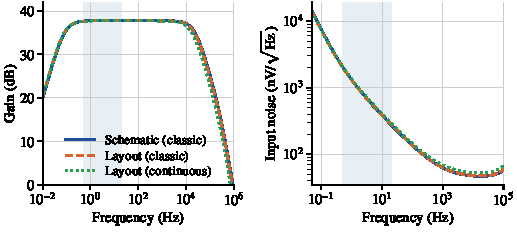
\includegraphics[width=\columnwidth]{figs/postlayout.pdf}
\caption{Gain and input-referred noise of the schematic and the extracted layout. The shaded band is the detector's 0.5--20\,Hz pass band.}
\label{fig:pl}
\end{figure}

Table~\ref{tab:cmp} compares the AFE with two classic designs. Integrated over the full 22-kHz bandwidth, the output noise referred to the input is about 10\uVrms, which with the whole circuit's 15.7\uA{} gives an NEF~\cite{steyaert1987} of about 10, against 4.0 for~\cite{harrison2003}. The white floor alone gives 9.2: only 4\uA{} of the 15.7\uA{} flows in the input pair, while the second stage takes 10\uA{} to drive the pin and its load. A lower second-stage current, which the EEG band permits, would lower the NEF and the power.

\begin{table}[t]
\caption{AFE Comparison}
\label{tab:cmp}
\centering
\footnotesize
\setlength{\tabcolsep}{3pt}
\begin{tabular}{@{}lccc@{}}
\toprule
 & This work & \cite{harrison2003} & \cite{verma2010} \\
\midrule
Process & SKY130 & 1.5\um{} & 0.18\um{} \\
Supply (V) & 1.8 & 5 & 1 \\
Gain (dB) & 37.8 & 39.5 & 60\textsuperscript{a} \\
Bandwidth & $<$0.15\,Hz--22\,kHz & 0.025\,Hz--7.2\,kHz & -- \\
Input noise (\textmu V\textsubscript{rms}) & 2.95 (0.5--100\,Hz) & 2.2 & 1.3 (100\,Hz) \\
Power (\textmu W) & 28\textsuperscript{b} & 80 & 3.5\textsuperscript{c} \\
NEF & $\approx$10 & 4.0 & -- \\
Area (mm$^2$) & 0.036\textsuperscript{d} & 0.16 & -- \\
Result & post-layout sim. & measured & measured \\
\bottomrule
\multicolumn{4}{@{}p{0.98\columnwidth}@{}}{\scriptsize \textsuperscript{a}Amplifier with its low-pass filter. \textsuperscript{b}Including bias and VREF. \textsuperscript{c}Low-noise amplifier stage. \textsuperscript{d}Whole 1$\times$2 tile.}
\end{tabular}
\end{table}

\subsection{Detection Performance and Implementation}

Table~\ref{tab:det} compares the detectors of the model search, all scored on the same folds, with the implemented detector. The built detector finds 47.8\% of seizures (95\% CI 34.5--60.4\%) at 0.91\,FA/h, detects at least one seizure in 33 of the 46 neonates with seizures and has a median latency of 35\,s; at the 0.5 and 2\,FA/h targets it finds 29.3\% and 58.1\%. Removing each detector's largest-contributing neonate changes the pre-declared, trees-only and CNN detectors by at most 2.8 points, against about a third for the two baselines. The CNN reference has the highest AUC and agreement but no higher event sensitivity than the trees-only procedure (49.8 versus 50.2\%), with about 300 times more operations per second. The RBF SVM is competitive in AUC, but its support vectors exceed the device's block RAM~\cite{amdk26} in three of five folds.

\begin{table}[t]
\caption{Detectors on Identical Nested Folds (79 Neonates, 1\,FA/h Target)}
\label{tab:det}
\centering
\footnotesize
\setlength{\tabcolsep}{2.1pt}
\begin{tabular}{@{}lccccc@{}}
\toprule
 & Median & Pooled & Sens.\ \% & Neonates & \\
Detector & AUC & AUC & (FA/h) & detected & $\kappa$ \\
\midrule
Threshold rule (first detector) & 0.734 & 0.700 & 26.6 (1.22) & 11/46 & 0.220 \\
RBF SVM & 0.839 & 0.837 & 44.3 (0.91) & 31/46 & 0.375 \\
Pre-declared procedure (all) & 0.827 & 0.790 & 31.7 (0.87) & 31/46 & 0.375 \\
Trees-only procedure & 0.868 & 0.800 & 50.2 (0.99) & 35/46 & 0.448 \\
CNN on raw EEG (reference) & 0.901 & 0.888 & 49.8 (1.10) & 39/46 & 0.573 \\
\textbf{Hardware-exact trees (built)} & \textbf{0.810} & \textbf{0.816} & \textbf{47.8 (0.91)} & \textbf{33/46} & \textbf{0.422} \\
\bottomrule
\multicolumn{6}{@{}p{0.98\columnwidth}@{}}{\scriptsize Linear, MLP and cost-aware configurations of the search are omitted.}
\end{tabular}
\end{table}

Trained on floating-point features, the same configuration gives paired differences whose 95\% confidence intervals all include zero: pooled AUC $+0.001$ [$-0.004$, $+0.005$], median AUC $+0.007$ [$-0.020$, $+0.029$], and sensitivity $0.0$ [$-1.1$, $+1.2$] points at 1\,FA/h and $-2.2$ [$-5.5$, $+0.2$] at 0.5\,FA/h. At 1\,FA/h the two alarm outputs agree in 99.63\% of seconds and detect the same 33 neonates, so defining the features in hardware arithmetic cost no measurable accuracy and the reported accuracy is that of the circuit.

After place and route (Vivado 2026.1, xck26-sfvc784-2LV-c) the detector uses 9,592 LUTs (8.2\%), 10,494 flip-flops (4.5\%), 62 DSP slices (5.0\%) and four 36-Kb block RAMs (2.8\%) and meets timing at 100\,MHz with 1.738\,ns of slack; its worst case of 2,399 cycles per time step is 0.61\% of the budget. The filters hold 60 of the 62 DSP slices. Four AFE channels draw about 0.11\,mW, against a vectorless estimate of 53\,mW for the detector logic, so the FPGA, not the front end, sets the power of the present system.

\subsection{AFE-to-Detector Interface}

\emph{Montage and noise.} Subtracting two single-ended channels adds their uncorrelated noise, so each bipolar derivation carries $\sqrt2 \times 2.44 = 3.5$\uVrms{} of AFE noise in the detector's 0.5--20\,Hz band (3.6\uVrms{} with the continuous models), roughly 20\uVpp. Healthy term background is mostly at or above 25\uVpp, and electrographic seizures range from a few to 150\uVpp{} or more~\cite{tsuchida2013}.

\emph{Common-mode rejection.} Re-referencing relies on matched gains. The within-die Monte Carlo gain spread of 0.06\% per channel gives $\sigma = 0.08$\% between two channels and a midband CMRR of about 62\,dB, including 50\,Hz, where the detector's notch adds further rejection; the gain is a capacitor ratio, but chip-to-chip spread is not modelled, and a per-channel digital gain calibration would remove the static part. Near $f_L$ pseudo-resistor differences dominate: with $f_L$ anywhere between 0.04 and 0.14\,Hz, the two responses differ by 20\% in magnitude and phase at 0.5\,Hz, only 14\,dB of rejection, rising to 34\,dB at 5\,Hz. Measuring each chip's $f_L$ and equalising it digitally would recover most of this.

\emph{Converter.} The linear output range is about $\pm0.39$\,V around VREF (5\,mV at the input); a 16-bit converter over this range has an input-referred step of 0.15\uV, negligible against the AFE noise. The 22-kHz AFE bandwidth, however, would fold white noise into the baseband if sampled directly at 256\,Hz, adding about 3.5\uVrms{} per channel within 0.5--20\,Hz (5\uVrms{} per bipolar derivation). A single-pole 40-Hz low-pass after the AFE ($-1$\,dB at 20\,Hz) makes the folded part negligible, as does a delta-sigma converter whose decimation filter rejects the band above 128\,Hz. For patient safety the acquisition board should be battery-powered and isolated.

\section{Discussion and Limitations}

Both halves are pre-silicon. Pseudo-resistors are poorly modelled and may differ by an order of magnitude on silicon, which would move $f_L$, and the AFE is specified for 0--50\,\textdegree C only, because pseudo-resistance falls and junction leakage grows exponentially above. On-board validation of the detector on the KV260, with measured latency and power, is in progress. The AFE is prepared for the Tiny Tapeout TTSKY26d shuttle, and gain, $f_L$, noise and artifact recovery will be measured on silicon.

The AFE noise is the main gap. The bipolar noise of about 20\uVpp{} suits medium- and high-amplitude discharges, but it is close to the 25-\textmu V\textsubscript{pp} lower limit of normal term background, above the smallest seizures~\cite{tsuchida2013} and an order of magnitude above clinical converters~\cite{ads1299}. The detector was evaluated on clinical recordings, so the effect of this noise on detection is not yet known; the next experiment adds the AFE's simulated noise and transfer function to the Helsinki recordings and repeats the nested evaluation. Chopper stabilisation or larger input devices would attack the $1/f$ noise.

The detector is not at expert level. Its agreement with the expert majority ($\kappa = 0.42$, 95\% CI 0.30--0.54) is well below that between the experts ($\kappa = 0.76$), 13 of the 46 neonates with seizures have none detected, and the per-neonate sensitivity is bimodal for every detector we tested. Software detectors report higher figures on their own data and protocols~\cite{temko2011,ansari2019,oshea2020}, which are not directly comparable. The implemented configuration (three channels, 8-s windows, 36 features) was fixed after the model search, on hardware-cost grounds and with outer-fold results known, which we disclose as a protocol amendment; the pre-declared trees-only procedure, fixed in advance, scored 50.2\%, so the late choice did not inflate the reported 47.8\%.

\section{Conclusion}

A capacitive-feedback EEG amplifier in SKY130 fits a 1$\times$2 Tiny Tapeout tile and has 2.95\uVrms{} of input noise in the EEG band at 28\uW{} in post-layout simulation, which also caught two parasitic couplings in its code-generated layout that rule and connectivity checks could not. A three-channel detector in the programmable logic of a Zynq UltraScale+ SoC, trained on its own integer features, matches its Python reference bit for bit and detects 47.8\% of seizures at 0.91 false alarms per hour on unseen neonates, in under 9\% of the device's logic and 24\,\textmu s per sample. The interface analysis shows that the AFE's $1/f$ noise and the chip-to-chip spread of its high-pass corner, not the converter or the detector's arithmetic, are the next limits to remove.

\section*{Acknowledgment}

The author used an AI assistant (Claude, Anthropic) for simulation and layout scripting, software development and manuscript drafting. All reported results come from the project repositories and their simulation and evaluation logs.

\bibliographystyle{IEEEtran}
\bibliography{refs}

\end{document}
